% this file is called up by thesis.tex
% content in this file will be fed into the main document

%: ----------------------- name of chapter  -------------------------
\chapter{SYSTEM OPERATION} % top level followed by section, subsection


%: ----------------------- paths to graphics ------------------------

% change according to folder and file names
\ifpdf
    \graphicspath{{4/figures/PNG/}{4/figures/PDF/}{4/figures/}}
\else
    \graphicspath{{4/figures/EPS/}{4/figures/}}
\fi

%: ----------------------- contents from here ------------------------
\section{Overview}
This chapter discusses pertinent operations of the system developed in this project work.

\section{System Operation}
When users visit the homepage of the web application, they are presented with a search form which allows them to enter both their \textit{departure} and \textit{destination} towns or cities. The applications takes text input, it then searches the routes database for routes containing searched text in departure and destination. The search results are displayed if routes exist,  displaying some information as shown in Figure \ref{fig:searchresults}. The routes departures and destinations have been geo-coded (converting the name or address of an area, point or route to the location; i.e. Latitude and Longitude) enabling user to have a fair idea of each route and stations location.\\

The user can view detailed information of each available routes, station and operator. The user also gets turn by turn routing information of each by selecting \textit{Go}, this is done by using the Open Source Routing Machine (OSRM) Application Programming Interface (API) which is embedded into OpenStreetMap as shown in Figure \ref{fig:routeinfo}, if done on a smartphone, location based applications could also be used. The user can also view departure and destination stations detailed information with an overview map below as shown in Figure \ref{fig:stationdown}; and can also geo located in OpenStreetMap or a location based mobile application by selecting \textit{Go} in Figure \ref{fig:stationtop}.

\section{Front End}
The front end consists of part of the system that can be viewed by visitors.
%\subsection{Homepage}
\begin{figure}[H]
	\centering
	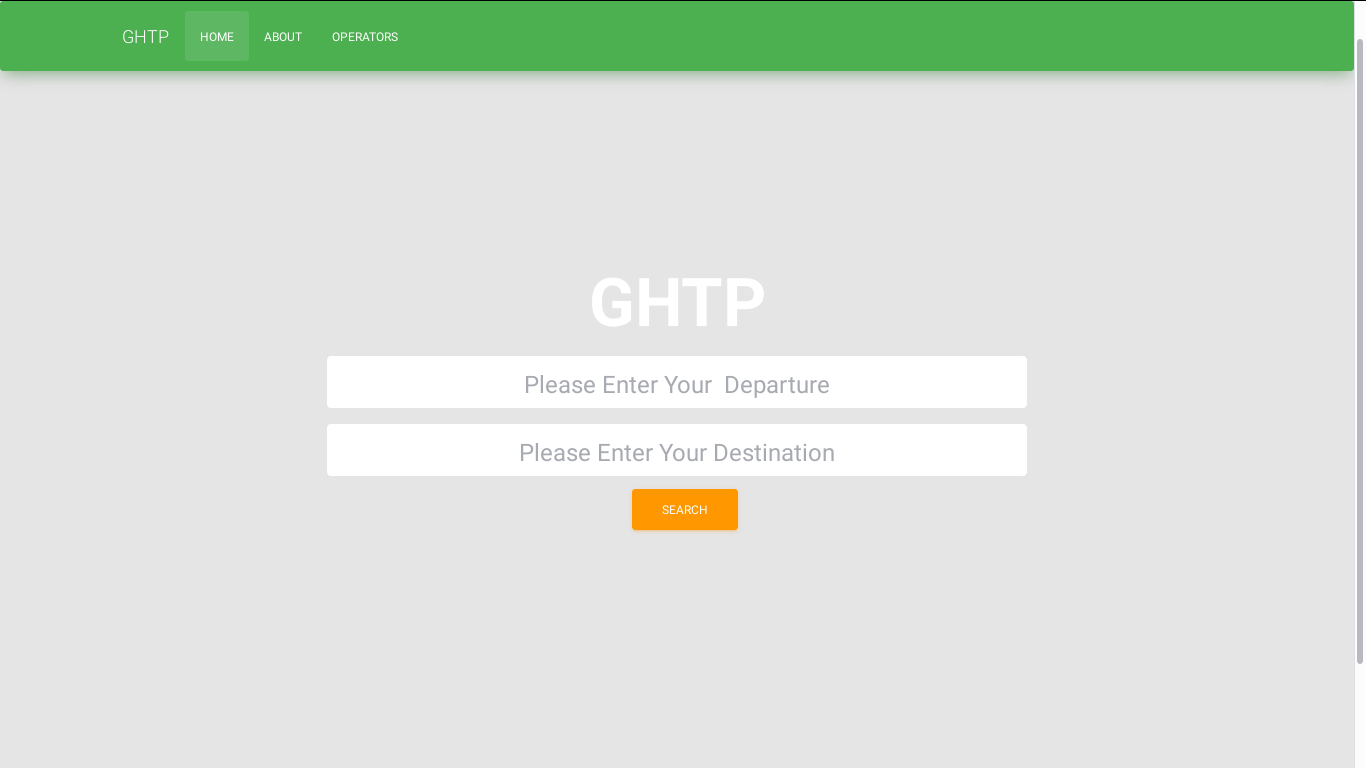
\includegraphics[width=1\linewidth]{hompage}
	\caption[Homepage]{Homepage}
	\label{fig:hompage}
\end{figure}
%\subsection{Search Results}
\begin{figure}[H]
	\centering
	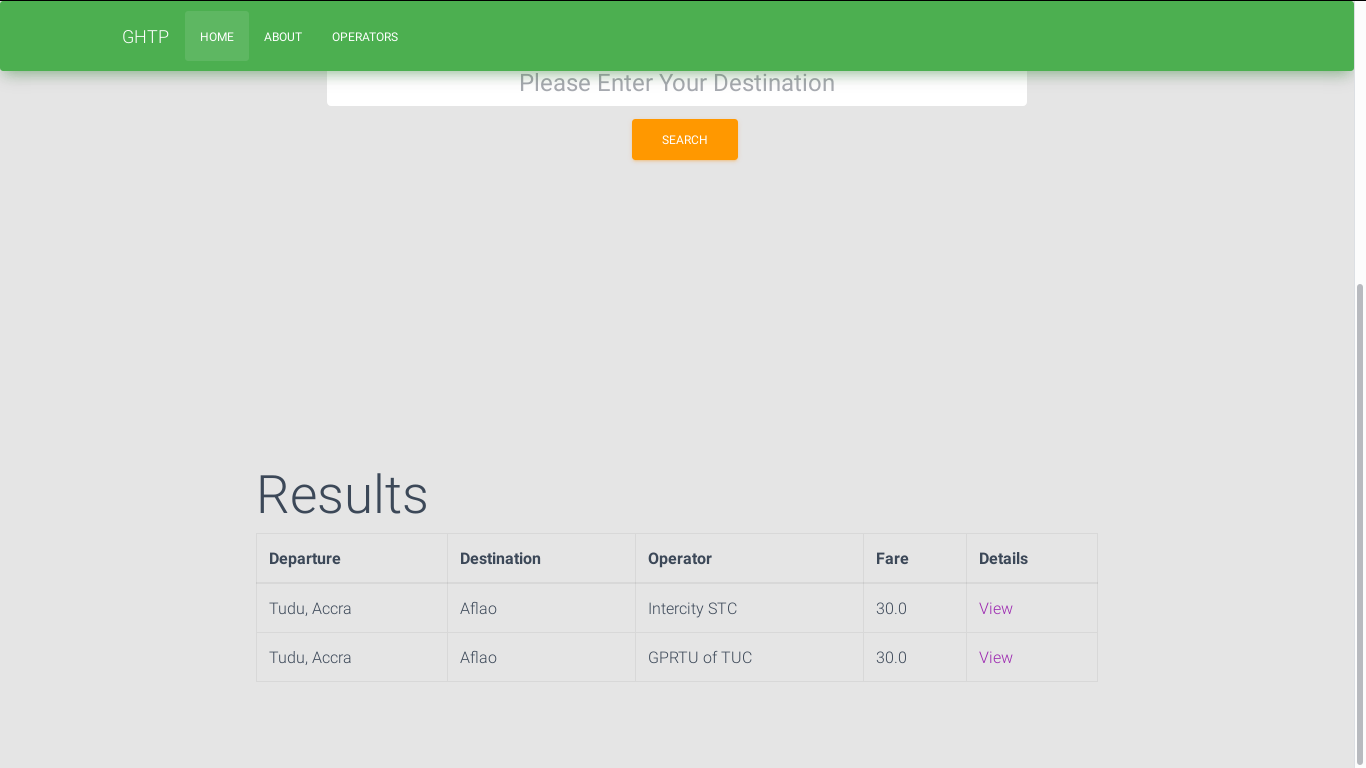
\includegraphics[width=1\linewidth]{searchresults}
	\caption[Search Results]{Search results}
	\label{fig:searchresults}
\end{figure}
%\subsection{Route Details}
\begin{figure}[H]
	\centering
	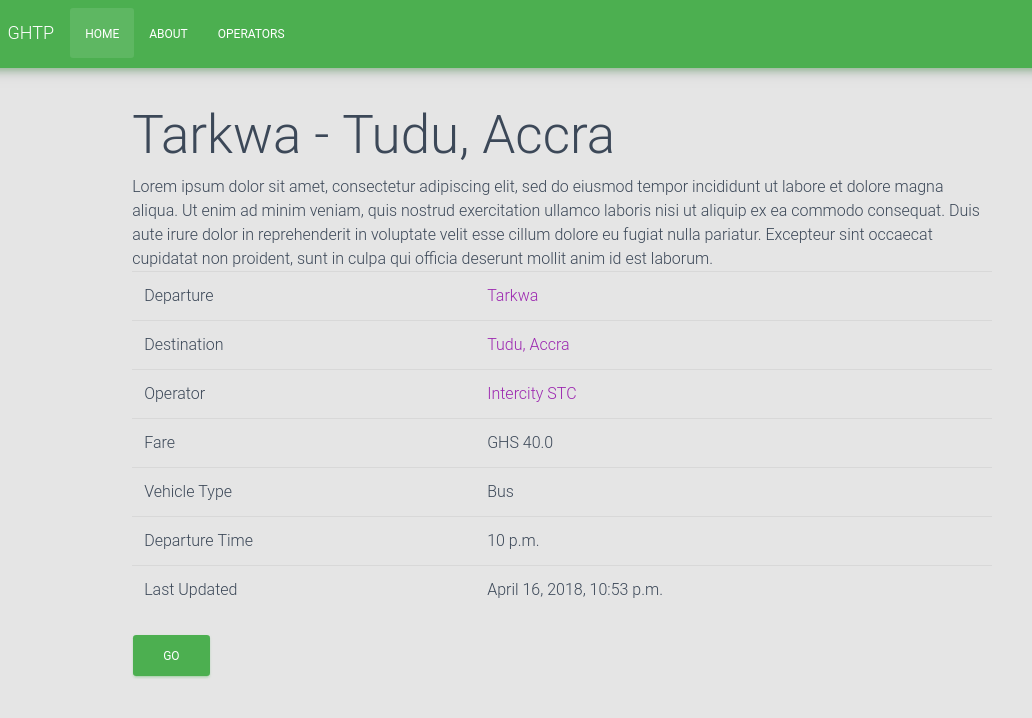
\includegraphics[width=1\linewidth]{routeinfo}
	\caption[Route Information]{Route information}
	\label{fig:routeinfo}
\end{figure}
%\subsection{Station Details}
\begin{figure}[H]
	\centering
	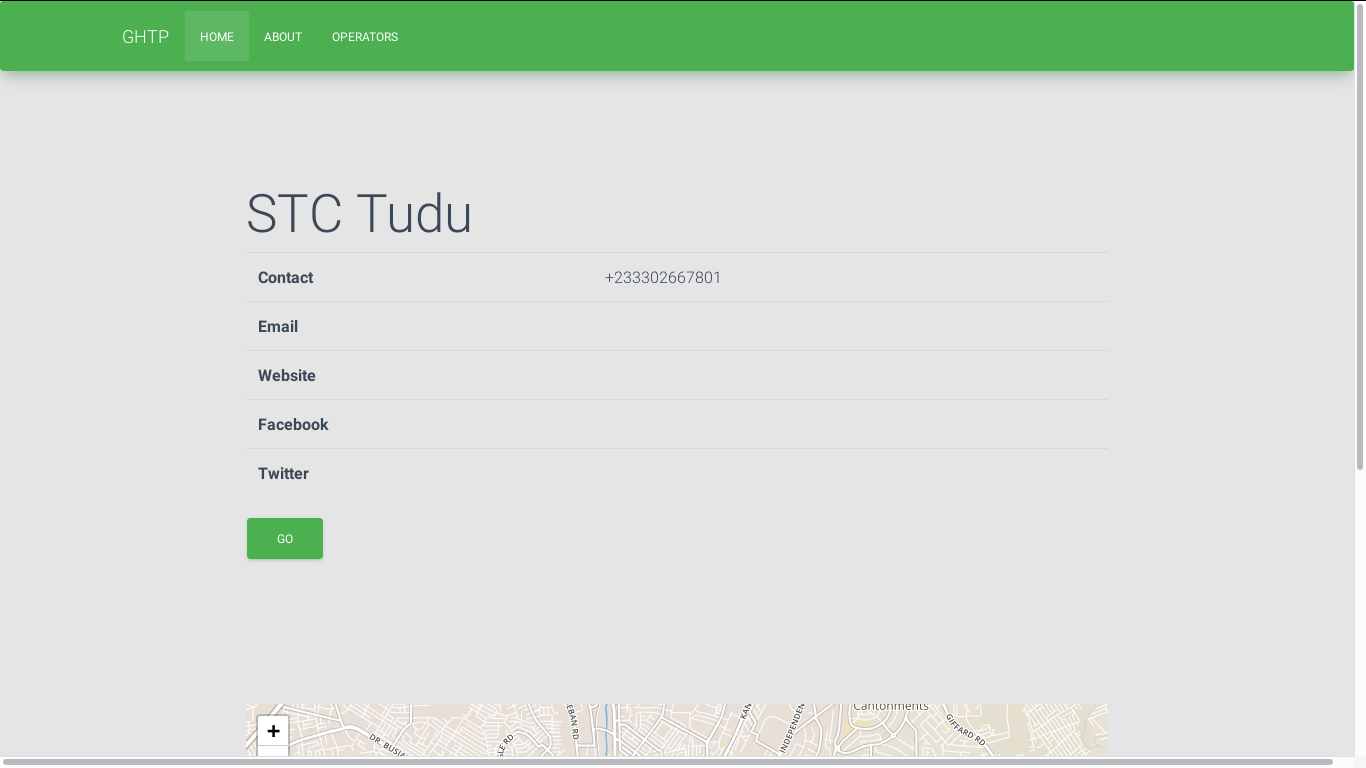
\includegraphics[width=1\linewidth]{stationtop}
	\caption[Station information]{Station information}
	\label{fig:stationtop}
\end{figure}
\begin{figure}[H]
	\centering
	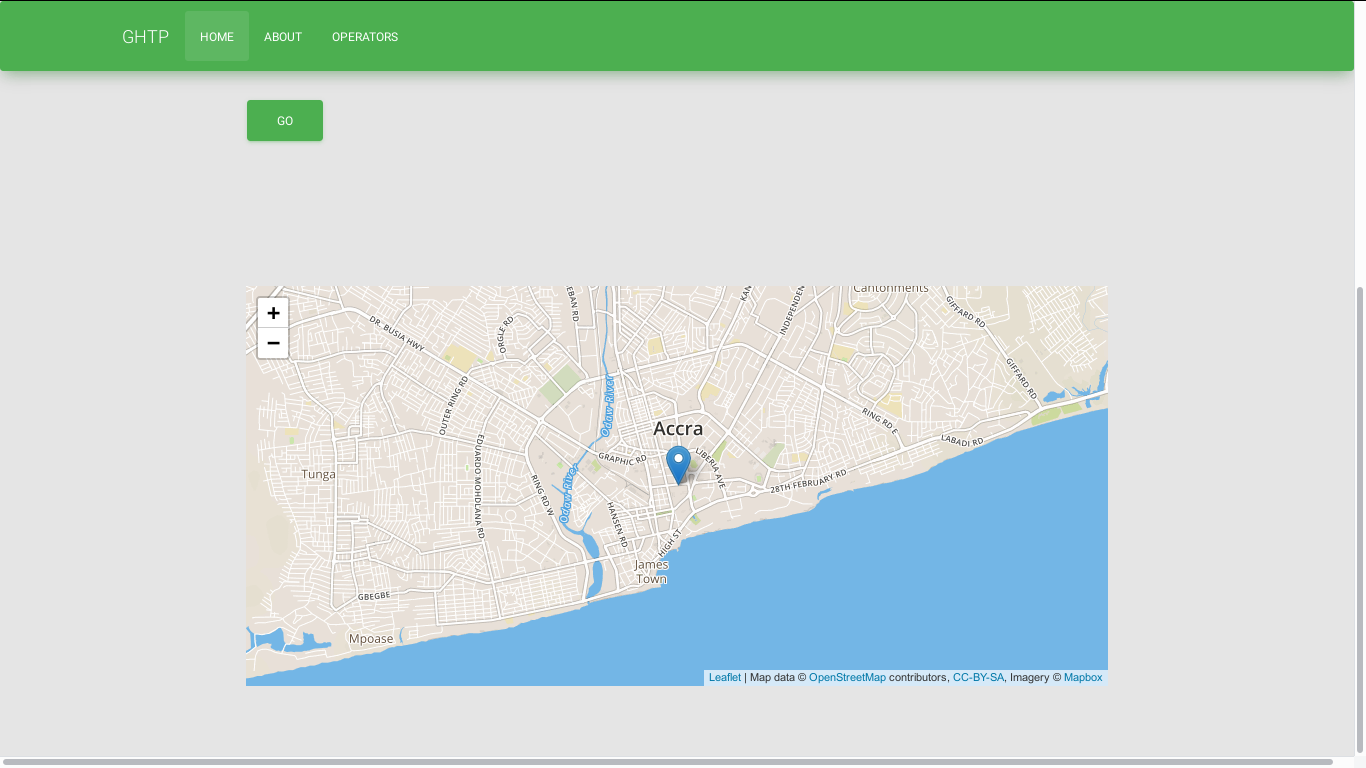
\includegraphics[width=1\linewidth]{stationdown}
	\caption[Station mini map]{Station location mini map}
	\label{fig:stationdown}
\end{figure}
%\subsection{Routing}
\begin{figure}[H]
	\centering
	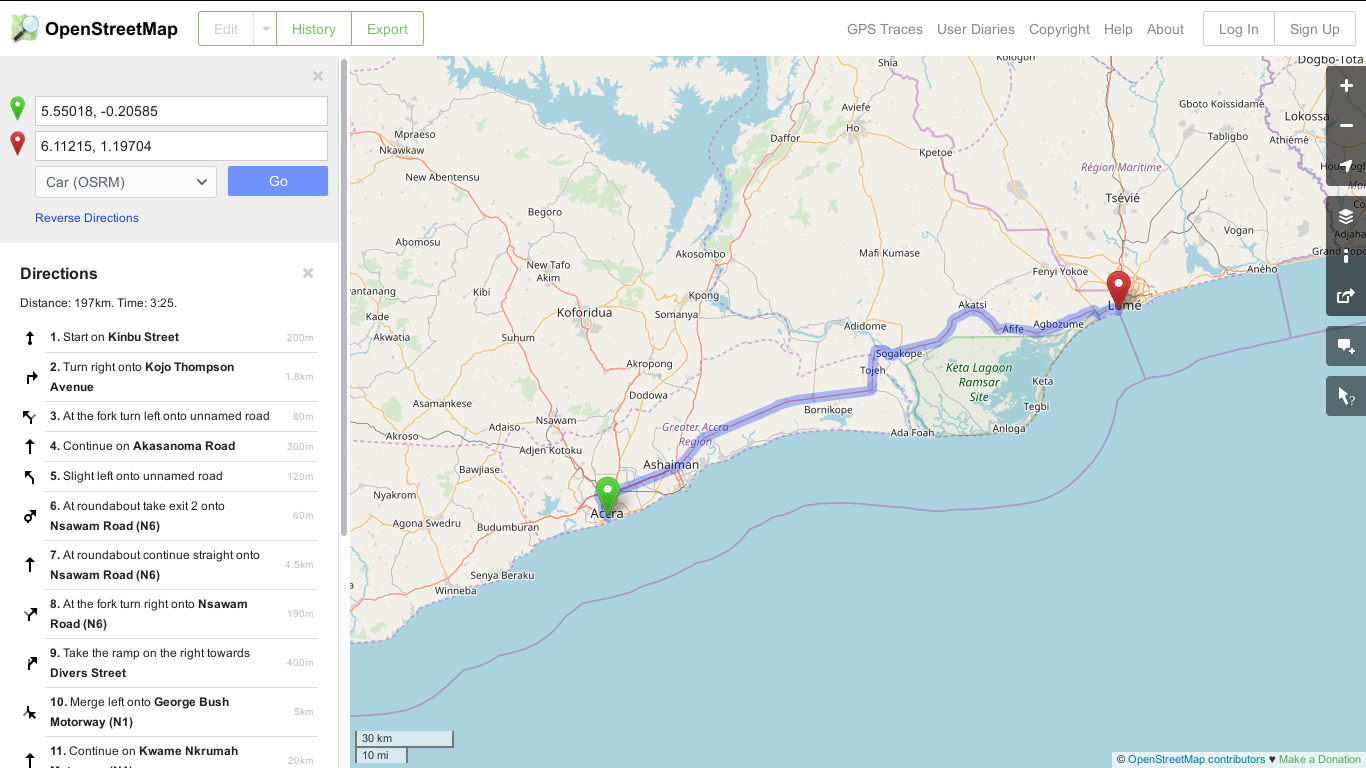
\includegraphics[width=1\linewidth]{routeosm}
	\caption[Turn by turn routing]{Turn by turn routing using OSRM API}
	\label{fig:routeosm}
\end{figure}
%\subsection{Available Operators}
\begin{figure}[H]
	\centering
	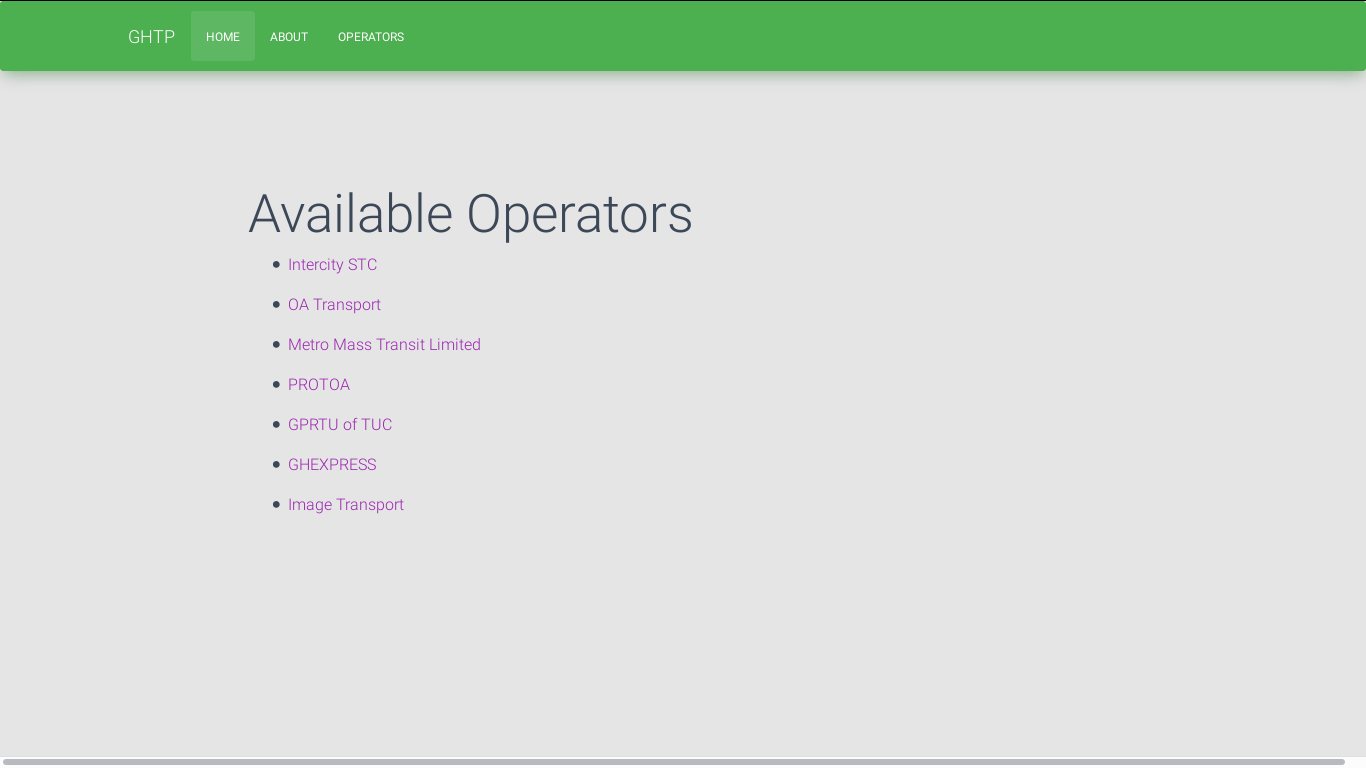
\includegraphics[width=1\linewidth]{availableoperators}
	\caption[Avalable operators]{Available transport operators}
	\label{fig:availableoperators}
\end{figure}

\section{Back End}
The back end is the administrative side of the system. Administrators and staffs with appropriated privileges can perform various functions such us adding, modify or deleting stations, operators, routes and staffs.
%\subsection{Login}
\begin{figure}[H]
	\centering
	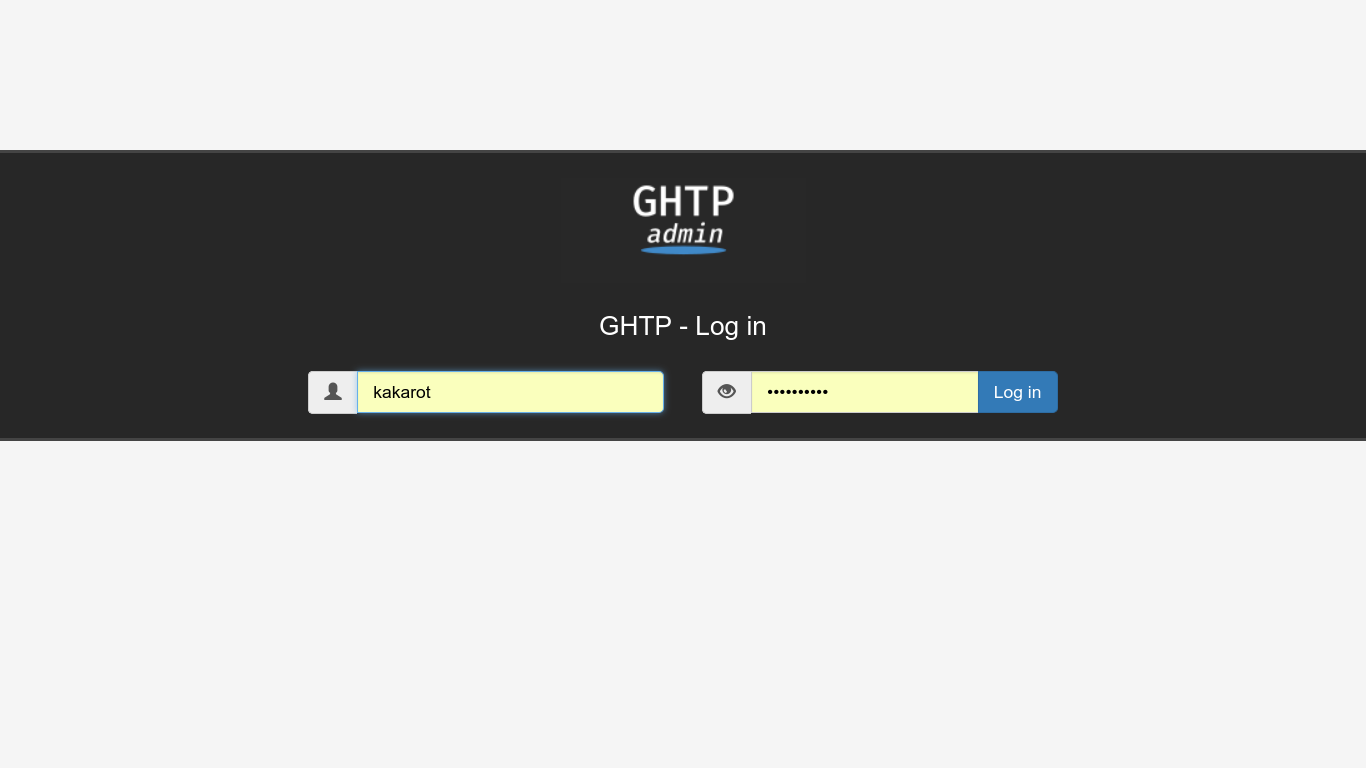
\includegraphics[width=1\linewidth]{adminlogin}
	\caption[Administration login]{Administration login}
	\label{fig:adminlogin}
\end{figure}
%\subsection{Administration Home}
The administration provides shortcuts to various features available and history of recent activities.
\begin{figure}[H]
	\centering
	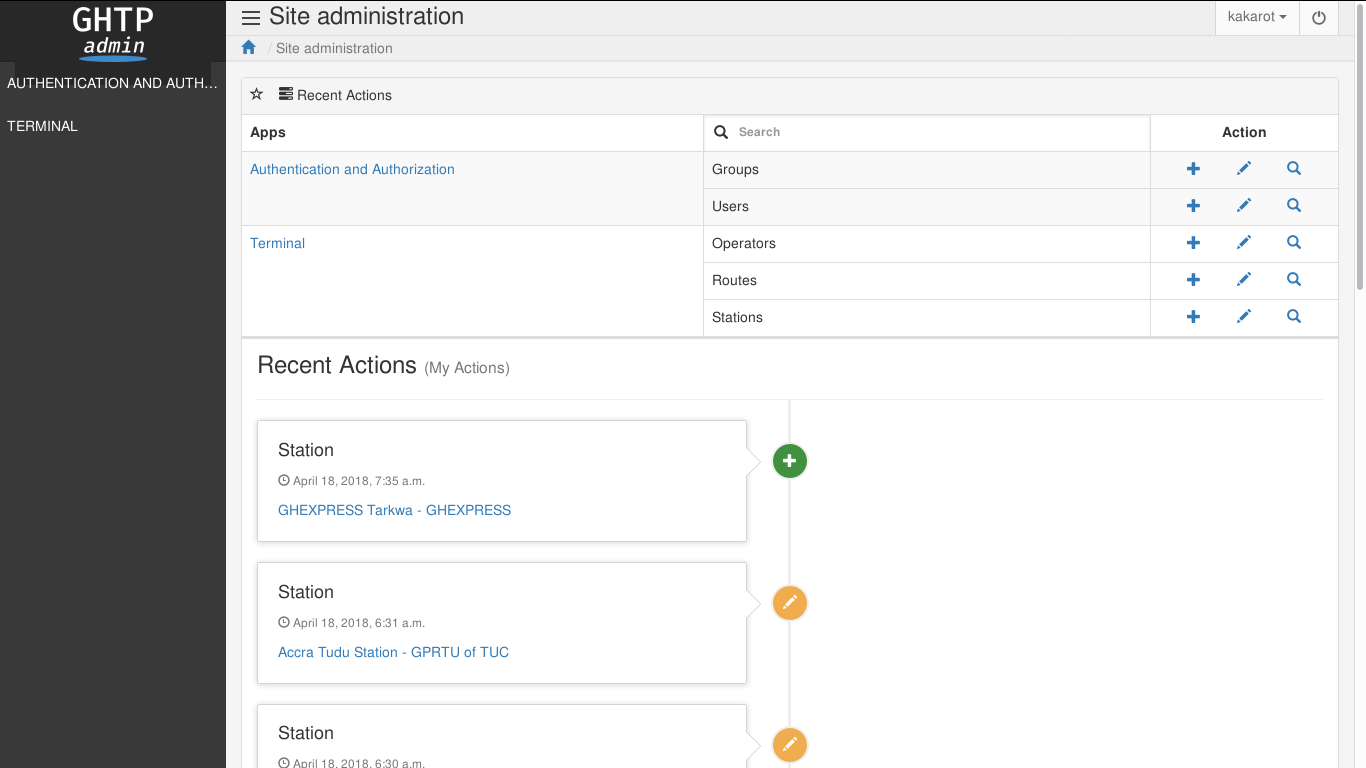
\includegraphics[width=1\linewidth]{adminhome}
	\caption[Administration dasboard]{Administration Dashboard}
	\label{fig:adminhome}
\end{figure}
%\subsection{Station Management}
\begin{figure}[H]
	\centering
	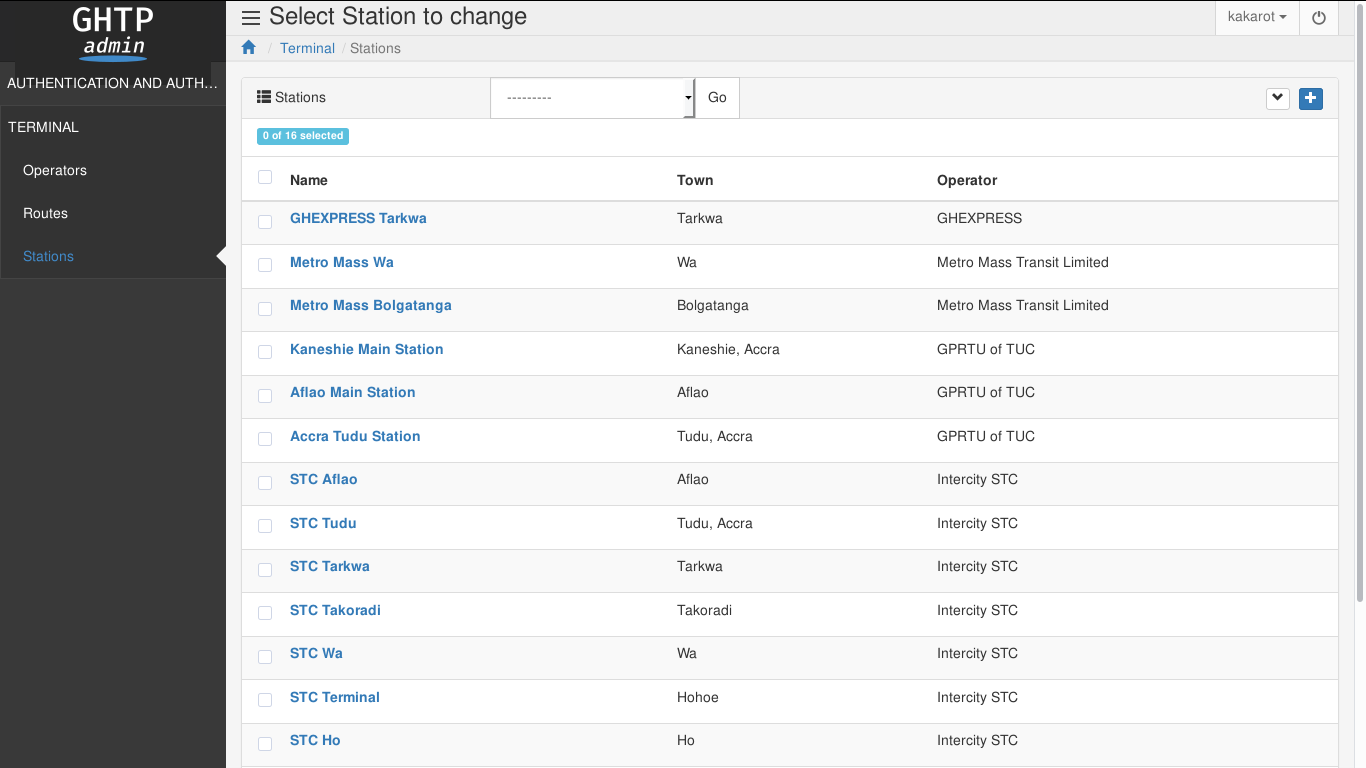
\includegraphics[width=1\linewidth]{stations}
	\caption[Managing stations]{Managing stations}
	\label{fig:stations}
\end{figure}
%\subsection{Operators Management}
\begin{figure}[H]
	\centering
	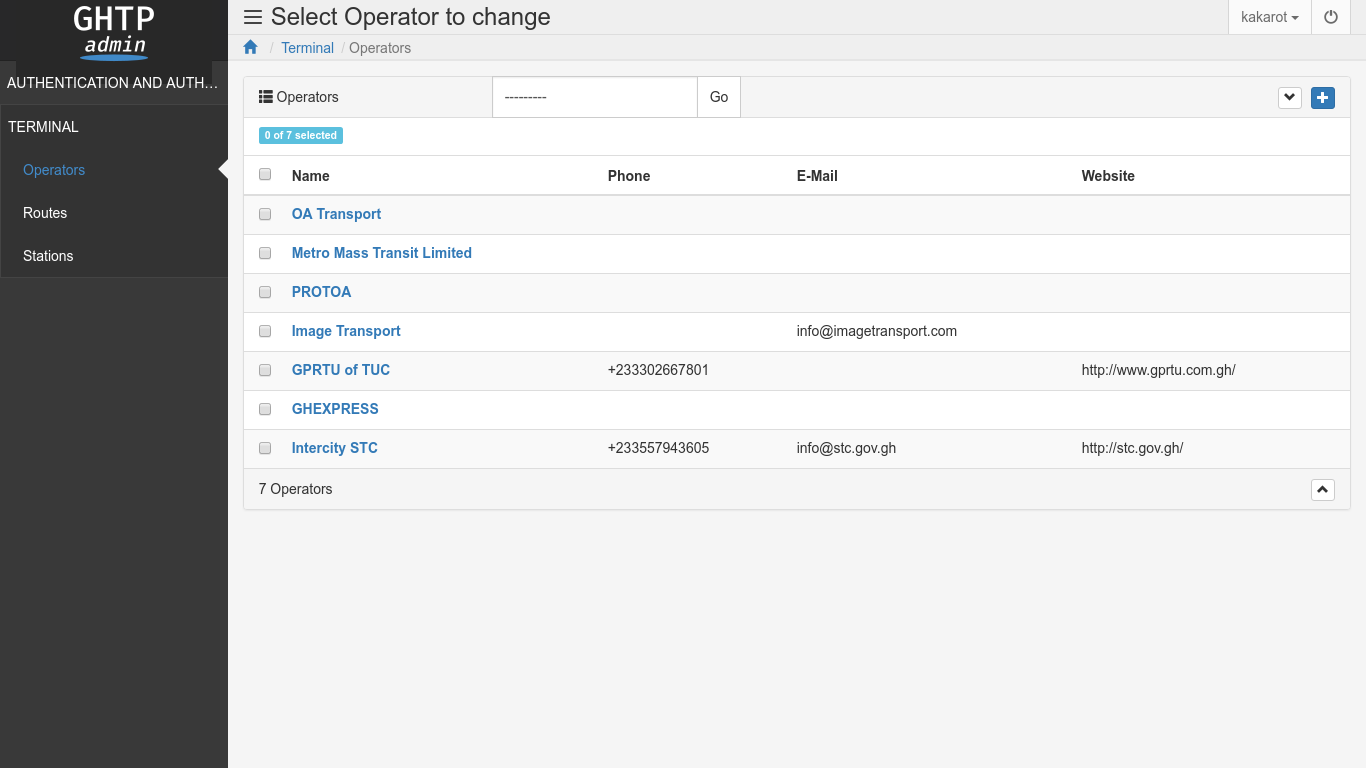
\includegraphics[width=1\linewidth]{operatorsadmin}
	\caption[Managing operators]{Managing operators}
	\label{fig:operatorsadmin}
\end{figure}
%\subsection{Route Management}
\begin{figure}[H]
	\centering
	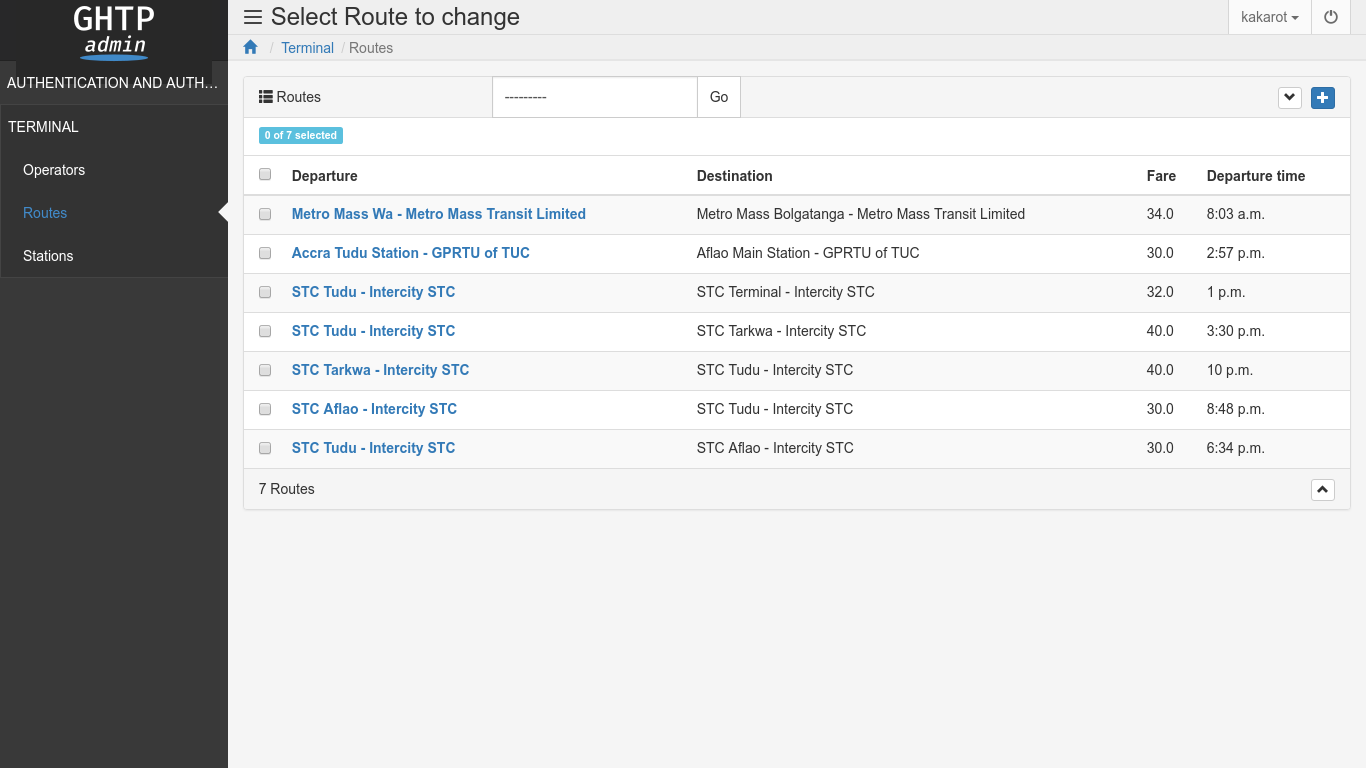
\includegraphics[width=1\linewidth]{routesadmin}
	\caption[Managing Routes]{Managing Routes}
	\label{fig:routesadmin}
\end{figure}
%\subsection{User Management}
\begin{figure}[H]
	\centering
	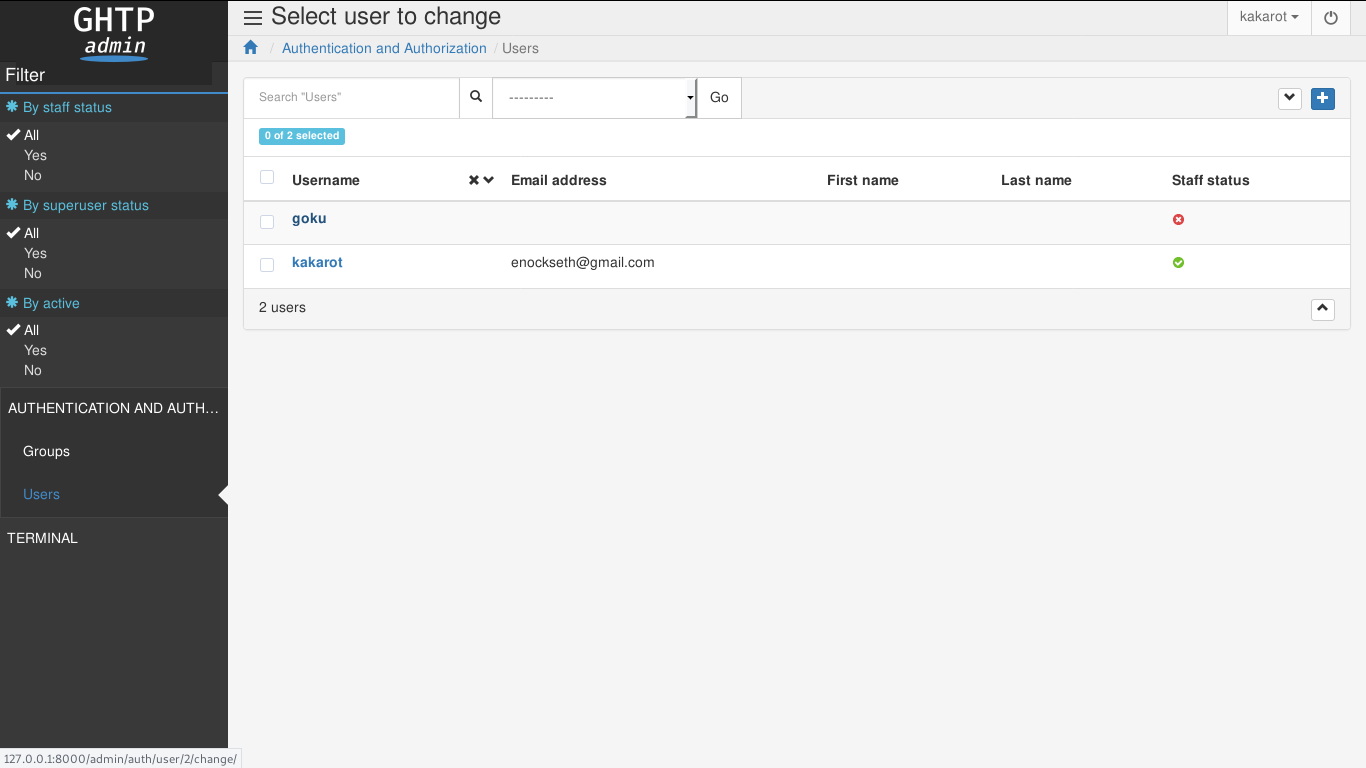
\includegraphics[width=1\linewidth]{usermanagement}
	\caption[Managing users]{Managing users}
	\label{fig:usermanagement}
\end{figure}





% ---------------------------------------------------------------------------
%: ----------------------- end of thesis sub-document ------------------------
% ---------------------------------------------------------------------------

